\documentclass[tikz,border=5mm]{standalone}
\usepackage{tikz}
\usetikzlibrary{arrows.meta, positioning, fit, calc}

\begin{document}
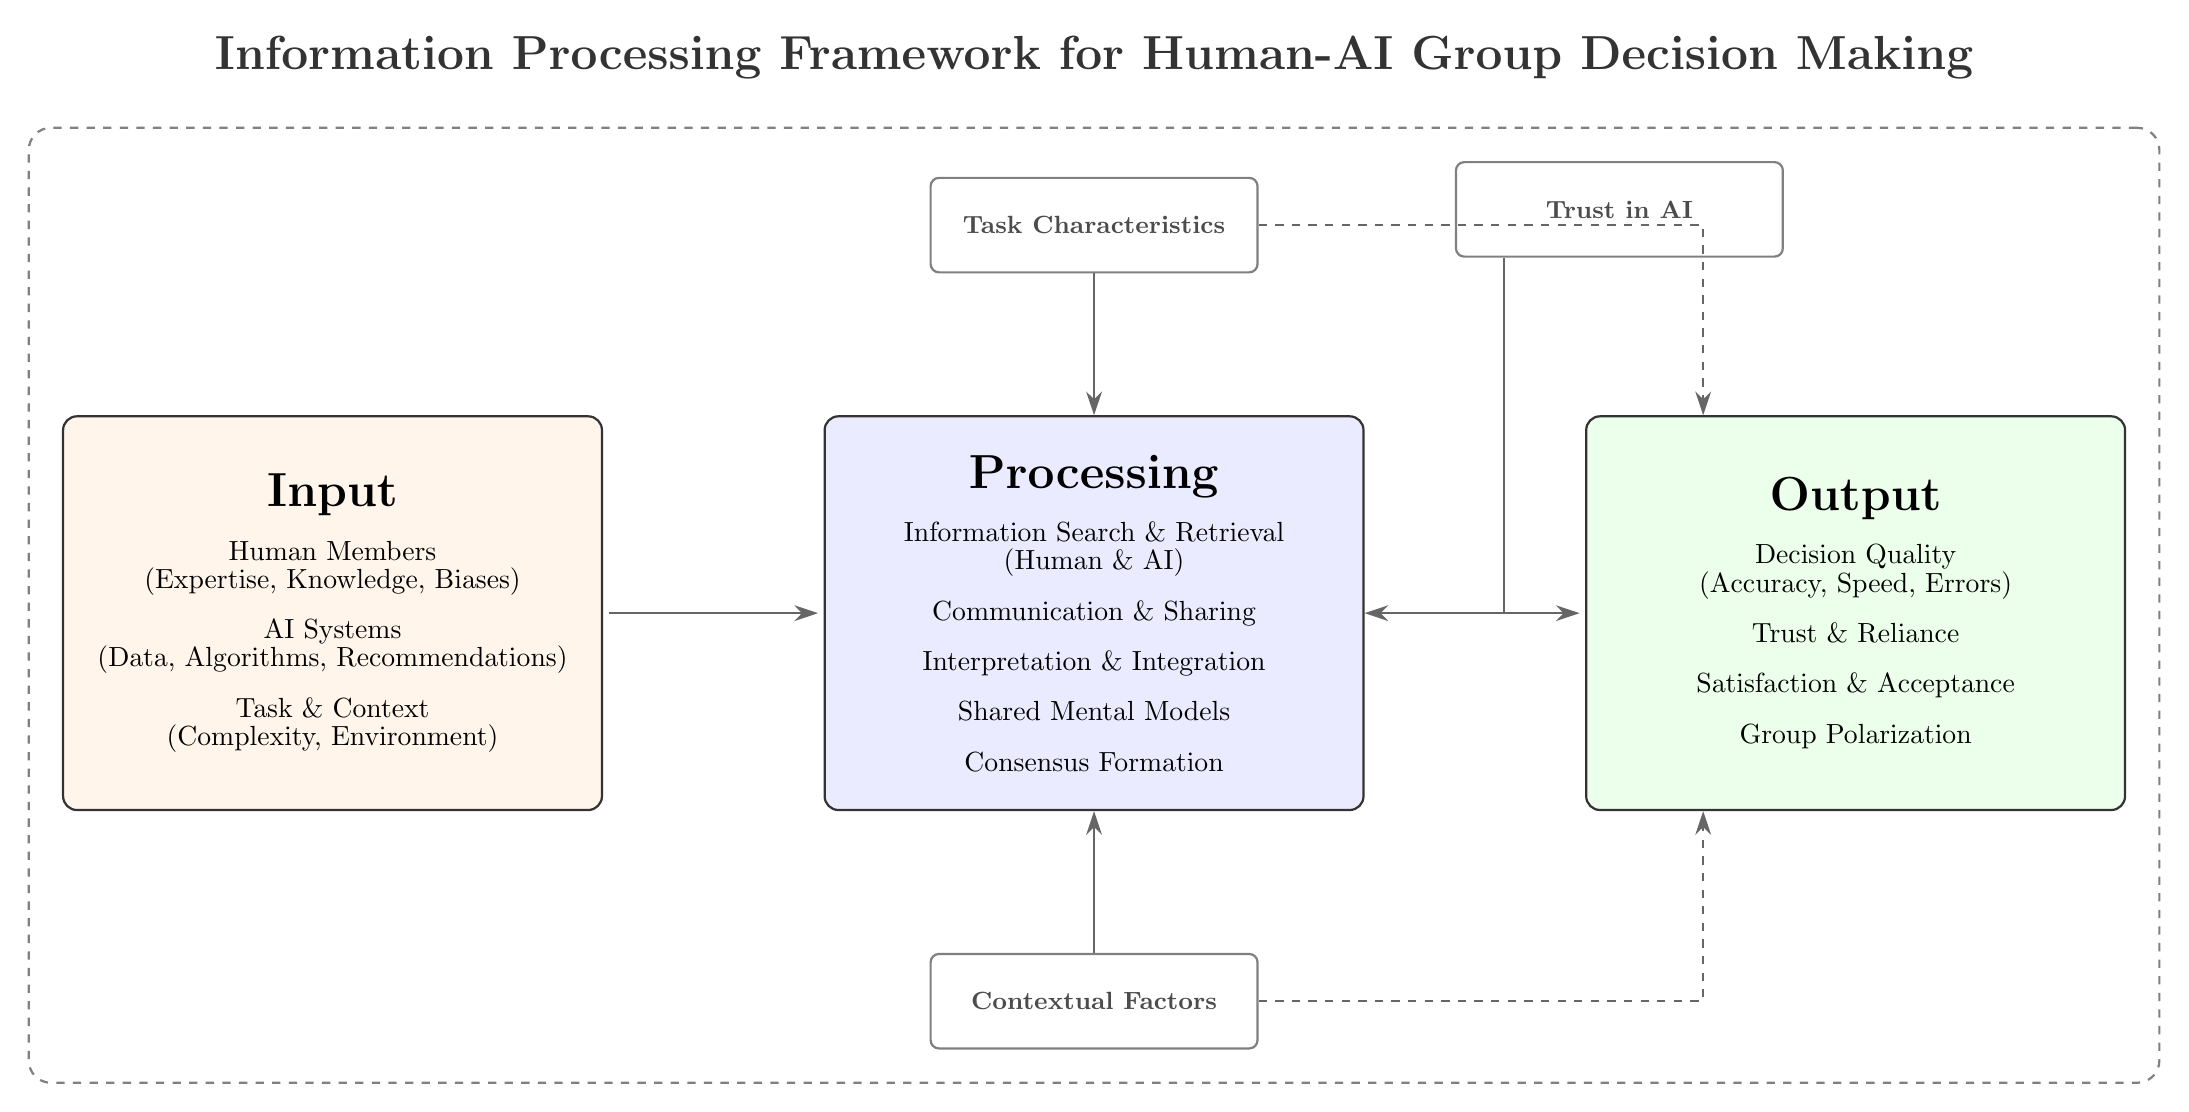
\begin{tikzpicture}[
    every node/.style={font=\normalsize\linespread{0.85}\selectfont}, % Base size increased to normal
    box/.style={
        rectangle, 
        rounded corners=5pt,
        draw=black!80,
        thick,
        align=center,
        inner sep=12pt
    },
    inputbox/.style={
        box,
        fill=orange!8,
        text width=6cm,
        minimum height=5cm
    },
    processbox/.style={
        box,
        fill=blue!8,
        text width=6cm,
        minimum height=5cm
    },
    outputbox/.style={
        box,
        fill=green!8,
        text width=6cm,
        minimum height=5cm
    },
    moderatorbox/.style={
        rectangle,
        rounded corners=3pt,
        draw=black!50,
        thick,
        fill=white,
        align=center,
        inner sep=5pt,
        text width=3.8cm,
        minimum height=1.2cm,
        font=\small\bfseries\color{black!70} % Moderator text now normal size
    },
    arrow/.style={
        thick,
        -{Stealth[length=3mm, width=2mm]},
        draw=black!60
    }
]

% Main IPO nodes
\node[inputbox] (input) {
    \textbf{\LARGE Input} \\[8pt] % Increased to LARGE
    Human Members \\ (Expertise, Knowledge, Biases) \\[8pt]
    AI Systems \\ (Data, Algorithms, Recommendations) \\[8pt]
    Task \& Context \\ (Complexity, Environment)
};

\node[processbox, right=2.8cm of input] (process) {
    \textbf{\LARGE Processing} \\[8pt] % Increased to LARGE
    Information Search \& Retrieval \\ (Human \& AI) \\[8pt]
    Communication \& Sharing \\[8pt]
    Interpretation \& Integration \\[8pt]
    Shared Mental Models \\[8pt]
    Consensus Formation
};

\node[outputbox, right=2.8cm of process] (output) {
    \textbf{\LARGE Output} \\[8pt] % Increased to LARGE
    Decision Quality \\ (Accuracy, Speed, Errors) \\[8pt]
    Trust \& Reliance \\[8pt]
    Satisfaction \& Acceptance \\[8pt]
    Group Polarization
};

% Moderator nodes
\node[moderatorbox, above=1.8cm of process] (moderator1) {Task Characteristics};
\node[moderatorbox, below=1.8cm of process] (moderator2) {Contextual Factors};
\node[moderatorbox, above=2cm of output, xshift=-3cm] (moderator3) {Trust in AI};

% Main flow arrows
\draw[arrow, shorten >=2pt, shorten <=2pt] (input) -- (process);
\draw[arrow, shorten >=2pt, shorten <=2pt] (process) -- (output);

% Moderator arrows
\draw[arrow] (moderator1.south) to[out=-90, in=90] (process.north);
\draw[arrow] (moderator2.north) to[out=90, in=-90] (process.south);

% Improved "Trust in AI" arrows
\draw[arrow] ($(moderator3.south west)!0.3!(moderator3.south)$) |- (process.east);

% Dashed influence arrows
\draw[arrow, dashed] (moderator1.east) -| ([xshift=15mm]output.north west);
\draw[arrow, dashed] (moderator2.east) -| ([xshift=15mm]output.south west);

% Framework bounding box
\node[draw=black!50, dashed, thick, rounded corners=8pt, 
       fit=(input) (process) (output) (moderator1) (moderator2) (moderator3),
       inner xsep=12pt, inner ysep=12pt] (frame) {};

% Title
\node[above=5mm of frame.north, anchor=south, 
       font=\bfseries\LARGE\color{black!80}, fill=white, inner sep=3pt] % Increased to LARGE
    {Information Processing Framework for Human-AI Group Decision Making};

\end{tikzpicture}
\end{document}